\chapter{Ingegneria dei requisiti}
\section{Requisiti}
Un requisito è una descrizione di una funzionalità che il sistema deve
fornire e le condizioni al contorno in cui tale sistema dovrebbe funzionare
(\textit{vincoli, operazioni, ...}).
Riflette quelle che sono le necessità del cliente e degli utenti finali del sistema 
software.

Si tratta di un problema  che all'origine sembra semplice, ma in realtà è molto
complesso.
\subsection{Requisiti utente e di sistema}

\begin{tcolorbox}[title ={User requirements}]
Si tratta di un requisito per come viene percepito dall'utente. Tipicamente
sono frasi in linguaggio naturale che esprimono le proprietà del sistema ed eventualmente 
con qualche diagramma per rendere più chiara la descrizione.

Tipicamente sono frasi astratte, e quindi non prevedono una soluzione.
\end{tcolorbox}
\begin{tcolorbox}[title ={System requirements}]
System requirements, ovvero i requisiti di sistema, sono requisiti più specifici,
strutturati e formali. Tipicamente sono espressi in un linguaggio formale, all'interno 
di un documento strutturato. Tipicamente il linguaggio è comprensibile anche 
da parte dell'utente, in modo che possa leggerlo e comprenderlo.
\end{tcolorbox}
Tipicamente i gli user requirements sono scritti dall'utente per avere un'idea 
di come il sistema dovrebbe funzionare. Essi possono essere la base per la formulazione di 
un contratto, dando quindi modo agli sviluppatori di definire le risorse necessarie
per lo sviluppo del sistema, abbozzando quindi un piano di lavoro.

I requisiti di sistema permettono di definire il sistema in modo più preciso,
in modo che i clienti possano validare ciò che il sistema deve fare.
\begin{tcolorbox}[title = {Stakeholders}]
Quando parliamo di requisiti, dobbiamo considerare gli stakeholder.
Gli stakeholder sono tutte quelle persone che hanno un interesse nel sistema, 
ovvero tutti gli utenti e tutti quelli che verranno toccati anche non 
interagendo con il sistema.
\end{tcolorbox}

Se venisse coinvolto un sottoinsieme di stakeholder, probabilmente alcune 
necessità verrebbero inespresse e di conseguenza implementate in modo parziale dal 
sistema software.
\subsection{Requisiti funzionali e non funzionali}
\begin{tcolorbox}[title = {Requisiti funzionali}]
Intendiamo che catturano le funzionalità che il sistema deve fornire, ovvero i servizi 
che deve mettere a disposizione che possono essere usati dagli utenti, come il sistema 
deve reagire a particolari eventi e come deve funzionare in particolari scenari. 
\end{tcolorbox}
I requisiti funzionali sono espressi mediante diversi livelli di astrazione e 
possibili ambiguità possono portare a diverse implementazioni. In caso di ambiguità è 
opportuno marcare il requisito come ambiguo, in modo che venga chiarito in seguito.

Oltre all'ambiguità, in relazione ai requisiti funzionali, si possono avere
diversi problemi. Prima di tutto bisogna cercare di raggiungere l'obiettivo legato 
alla \textbf{completezza}, ovvero che tutte le funzionalità siano state catturate
dai requisiti. Il secondo obiettivo è quello della \textbf{consistenza}, ovvero che
non ci siano requisiti che si contraddicono tra loro.

Nella pratica è difficile raggiungere questi obiettivi, perché stakeholder diversi
potrebbero avere opinioni diverse su come il sistema dovrebbe funzionare, e quindi
potrebbero esserci delle contraddizioni. Inoltre, potrebbero esserci imprecisioni
e ambiguità tramite clienti e sviluppatori.

Alcune inconsistenze potrebbero sfuggire durante la fase di analisi dei requisiti,
e potrebbe emergere quando tale requisito deve essere implementato correttamente.

\begin{tcolorbox}[title = {Requisiti non funzionali}]
I requisiti non funzionali sono tutti quei requisiti che non sono legati alle
funzionalità del sistema, ma che riguardano le proprietà del sistema.
\end{tcolorbox}
Tipicamente sono vincoli legati al sistema e non sono legati al singolo componente 
del sistema.

Il problema è che tali requisiti non emergono in maniera spontanea da una frase pronunciata dal 
nostro cliente, perché tipicamente gli utenti hanno in mente le funzionalità del sistema
e non le proprietà del sistema. Potrebbe quindi aiutare l'avere una tassonomia legata a 
quali sono i requisiti non funzionali, in modo da poterli riconoscere e quindi
poterli catturare.
\begin{figure}[H]
    \centering
    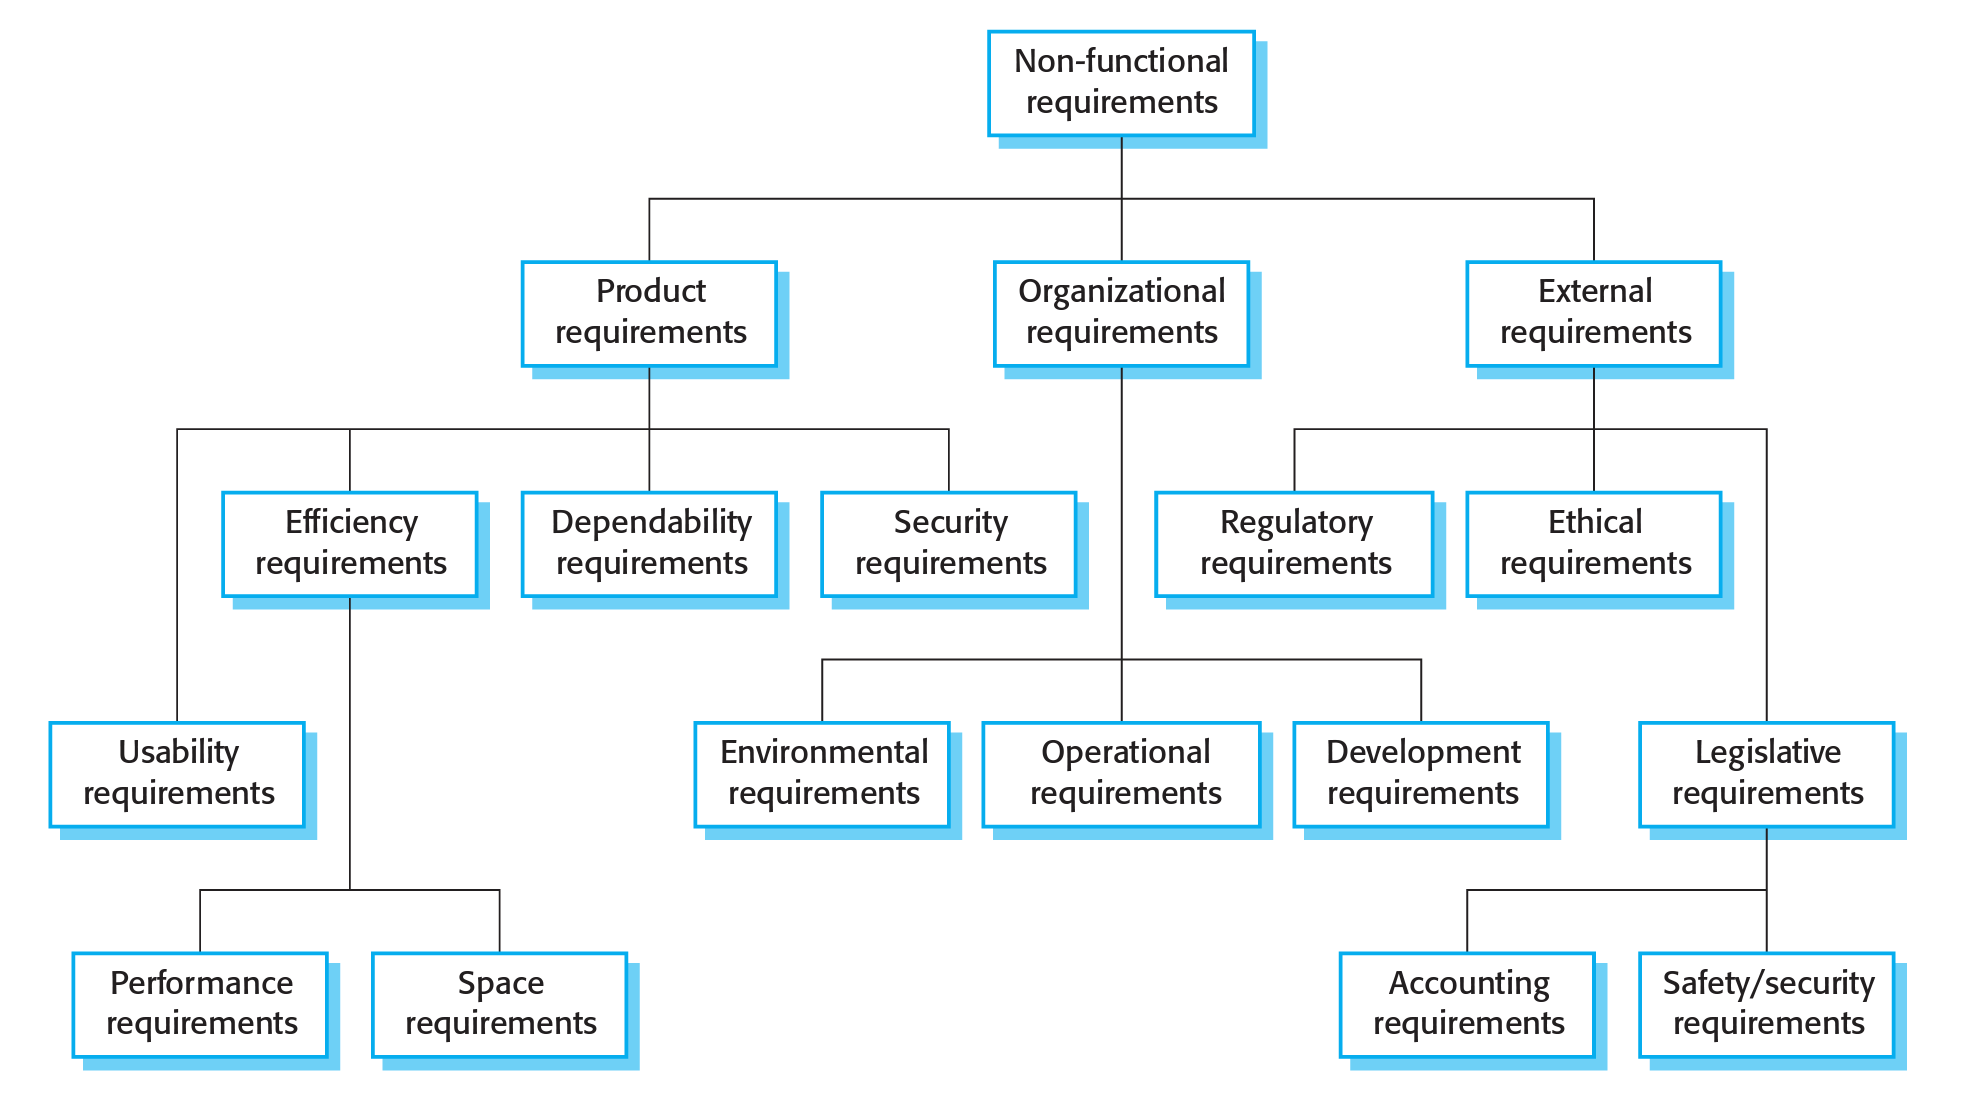
\includegraphics[scale=0.4]{img/nonfunctional.png}
\end{figure}
\subsection{Verifica dei requisiti non funzionali}
Siccome i vincoli non funzionali sono di alto livello, potrebbe risultare abbastanza difficile 
capire se sono soddisfatti o meno. Sarebbe opportuno quindi scrivere tali requisiti in maniera più 
quantitativa possibile invece che qualitativa. 
Supponiamo di disporre di tale vincolo:
\begin{tcolorbox}
    Il sistema deve essere facile da usare da parte dello staff medico in modo da minimizzare gli errori.
\end{tcolorbox}
Ma come facciamo a capire se il sistema è facile da usare? È opportuno quindi
trasformare da qualitativo a quantitativo, in modo da poterlo misurare.
\begin{tcolorbox}
    Il sistema deve essere facile da usare da parte dello staff medico in modo da minimizzare gli errori. 
    Il sistema deve essere usabile da parte di un medico con meno di $4$ ore di formazione.
    Il numero medio di errori per ora di utilizzo non deve superare $2$ per ora.
\end{tcolorbox}
Fondamentale quindi è la capacità di tradurre i requisiti non funzionali qualitativi in 
requisiti non funzionali quantitativi, in modo da poterli misurare e quindi verificare, anche mediante 
metriche.

\section{Processi di ingegneria dei requisiti}
Di fatto ci sono tre fasi nella gestione dei requisiti:
\begin{itemize}
    \item \textbf{Elicitazione dei requisiti}: si cerca di capire quali sono i requisiti,
    in modo da poterli catturare e quindi poterli documentare. Dove l'output è la 
    descrizione del sistema.
    \item \textbf{Specifica dei requisiti}: ovvero come vengono scritti tali requisiti.
    Dove l'output sono i requisiti dell'utente e del sistema.
    \item \textbf{Validazione dei requisiti}: si verifica che i requisiti siano completi e 
    non contradditori. Dove l'output è il documento dei requisiti.
\end{itemize}
\begin{figure}[H]
    \centering
    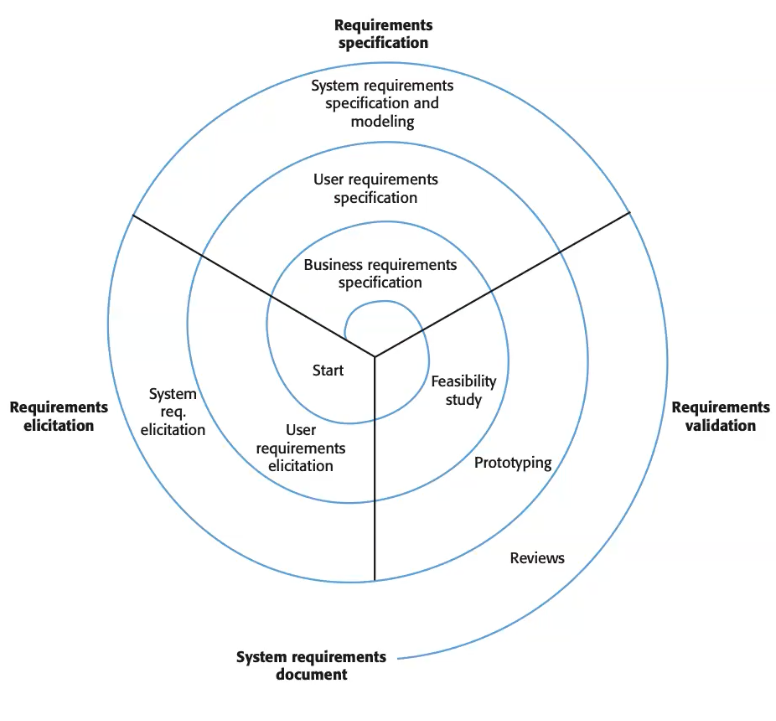
\includegraphics[scale=0.4]{img/requisitispirale.png}
\end{figure}
In generale, il processo di sviluppo può essere descritto come un ciclo a spirale.
Inizia con la specifica dei
requisiti, in cui si definiscono i business requirements iniziali, ovvero i
requisiti legati al dominio applicativo. Dopo, si passa alla validazione dei
requisiti, verificando la loro completezza e coerenza.

Si riparte con la elicitazione dei requisiti, dove con la ripetizione di
questo processo, emergono nuovi requisiti legati agli utenti. Questo permette
di aggiornare la specifica dei requisiti utente e procedere con la loro validazione.
Il ciclo si ripete ancora, focalizzandosi sui requisiti di sistema.

\subsection{Elicitazione dei requisiti}
Gli sviluppatori devono capire il dominio applicativo, le funzionalità
che il sistema dovrà fornire, e i vincoli non funzionali come le performance
e l'interazione con l'hardware. Possono presentarsi ostacoli: per esempio, i
clienti potrebbero esprimere i requisiti usando termini non noti agli ingegneri
del software o dare per scontati alcuni aspetti che sono ovvi nel loro dominio
applicativo, oppure i requisiti potrebbero essere irrealizzabili.

La presenza di diversi stakeholder può portare a differenti obiettivi, risultando
in requisiti potenzialmente in conflitto. La collaborazione può essere compromessa
se gli stakeholder non si sentono rappresentati e possono emergere fattori politici.
I requisiti potrebbero cambiare o emergere nel corso dello sviluppo.
\subsubsection{Intervista}
Un metodo primario per raccogliere i requisiti è l'intervista, che può includere
domande sia chiuse che aperte, generalmente in una forma mista. Tuttavia, gli
stakeholder non sempre forniscono requisiti dettagliati.

È importante condurre
le interviste in modo efficace, cercando di evitare pregiudizi e verificando le
proprie assunzioni. È consigliabile iniziare con domande semplici, evitando di
partire subito con concetti troppo astratti.

I problemi che possono verificarsi sono legati alla difficoltà di capire
il dominio applicativo, e quindi di catturare i requisiti. Una determinata classe 
di medicinali per un medico potrebbe essere ovvia, ma non per un ingegnere del software,
non sentendo quindi il bisogno di descriverlo nei requisiti. Inoltre, potrebbero
esserci dei problemi aziendali che portano gli stakeholder a non voler
condividere informazioni, o a non voler cambiare i processi aziendali.

I suggerimenti sono quindi di lavorare con mentalità aperta, cercando di
capire il dominio applicativo, e di non dare per scontato nulla ed evitare 
domande preconfezionate. 
\subsubsection{Etnografia}
Non intervistare le persone, ma lavorare insieme a loro, per capire il loro
necessità. Questo aiuta molto la conoscenza implicita che potrebbe non emergere 
durante l'intervista. Questo tipo di studio può essere attuato con un sistema software 
esistente, oppure se l'azienda ha già un'operatività anche cartacea.
\subsubsection{Storie e Scenari}

\paragraph{Storie} Le storie sono narrazioni ad alto livello che forniscono
esempi concreti del funzionamento del sistema software in un contesto specifico.
Sono formulate in modo narrativo e facile da comprendere, e permettono agli
stakeholder di visualizzare l'interazione con il sistema e di esprimere feedback
su ciò che ritengono appropriato o meno.

\paragraph{Scenari} Gli scenari, invece, rappresentano esempi di utilizzo
più dettagliati del sistema. Descrivono un'interazione specifica tra l'utente
e il sistema, includendo dettagli come l'input specifico. Questo li rende strumenti
più precisi per illustrare le funzionalità del sistema e per validare i requisiti
con gli stakeholder.


Una storia raccoglie può quindi raccogliere più scenari.
\subsection{Specifica dei requisiti}
La specifica dei requisiti è il processo di scrittura dei requisiti in un
documento. I requisiti devono essere scritti in modo chiaro e preciso, in modo
da essere comprensibili a tutti gli stakeholder. 
Gli user requirements devono essere comprensibili per gli utenti, mentre i system
requirements possono includere dettagli tecnici. Tale documento può essere 
parte del contratto tra cliente e fornitore, e può essere usato come base per
la verifica e la validazione dei requisiti, devono quindi essere più completi 
possibili.

In linea di principio viene descritto \textbf{cosa} il sistema dovrà fare non contenendo
dettagli implementativi. In pratica però, è difficile separare i requisiti e 
potrebbero quindi emergere dettagli implementativi, legati anche all'architettura. 
\subsubsection{Linguaggio naturale}
Il primo modo per scrivere i requisiti è il linguaggio naturale, che però è
intrinsecamente ambiguo. Per ridurre l'ambiguità, si possono usare i verbi modali
in modo corretto, e usare il grassetto per evidenziare parti chiave.

Si evita di norma l'utilizzo di gergo tecnico, e si usano invece termini
che gli stakeholder possono comprendere. Di norma quando un requisito è
inserito all'interno è accompagnato dalla motivazione per cui è necessario.
\subsubsection{Struttura vincolata}
Un altro modo per scrivere i requisiti è la struttura vincolata, che permette
di avere una struttura standard per i requisiti. Questo permette di avere
una struttura standard, ma non è sempre facile da usare e può essere limitante.
\subsubsection{Use cases}
L'use case è una descrizione di un insieme di sequenze di azioni che un sistema
e serve per identificare gli attori e le funzionalità del sistema che fanno 
riferimento ai vari utenti.
\begin{figure}[H]
    \centering
    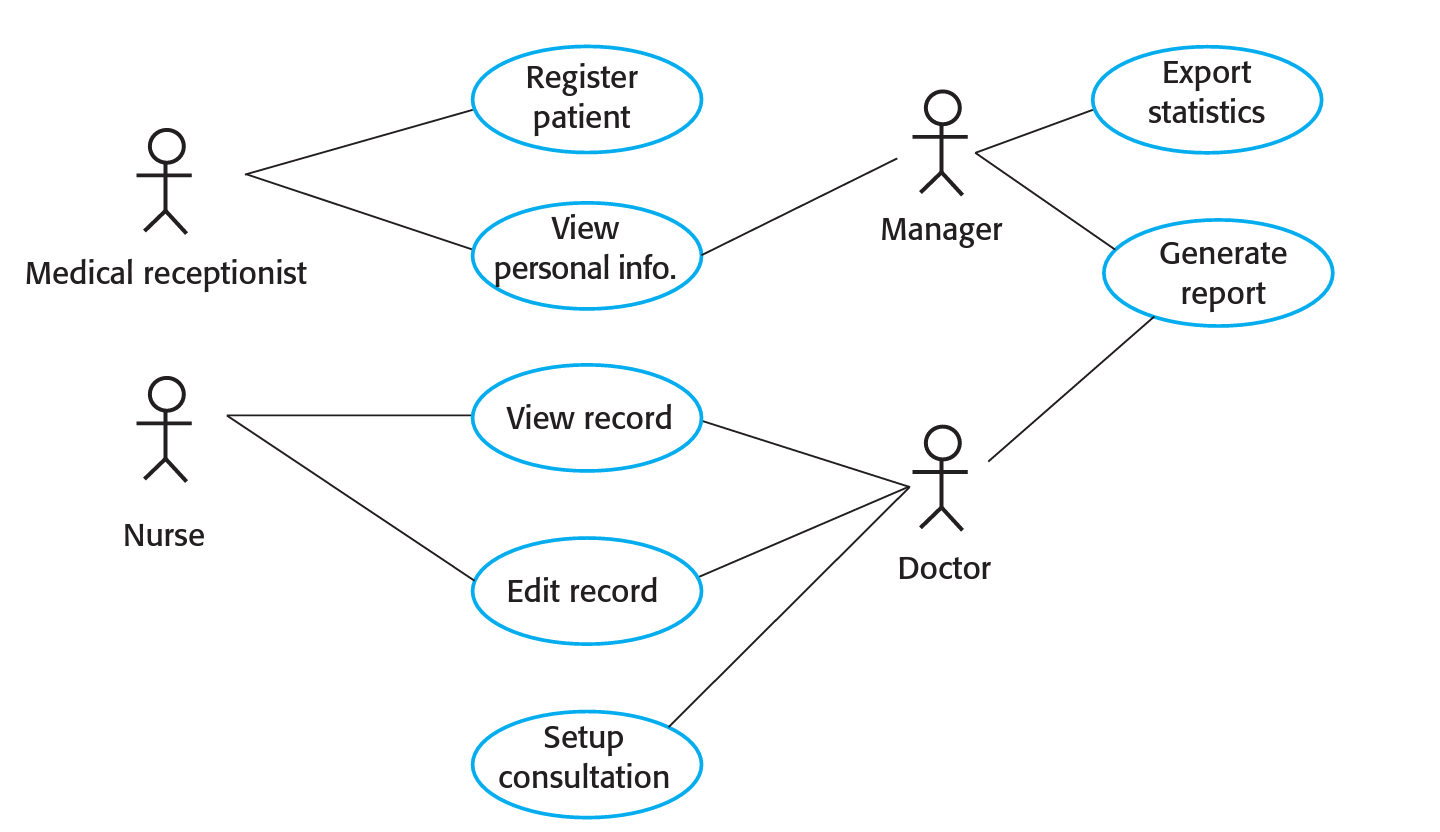
\includegraphics[scale=0.4]{img/usecase.png}
\end{figure}
\subsubsection{Documento dei requisiti}
Il \textbf{Documento dei Requisiti Software} è fondamentale per la specificazione
dei requisiti. Questo documento può variare a seconda delle organizzazioni e dei
contesti; tuttavia, esistono standard definiti da organizzazioni internazionali
che possono fornire linee guida e struttura. Un esempio di tale standard è quello
proposto dall'\texttt{IEEE} (\textit{Institute of Electrical and Electronics Engineers}).
\subsection{Validazione dei requisiti}
L'obiettivo principale della validazione dei requisiti software è assicurare
che i requisiti definiti corrispondano effettivamente al sistema desiderato dal
cliente. È particolarmente costoso rilevare difetti nei requisiti nelle fasi avanzate
dello sviluppo, arrivando a costi fino a $100$ volte superiori.

Una checklist efficace per la validazione dei requisiti include i seguenti punti:
\begin{itemize}
    \item \textbf{Validità:} Il sistema fornisce le funzionalità che meglio supportano
    le necessità del cliente?
    \item \textbf{Consistenza:} Ci sono conflitti tra i requisiti (\textit{contraddizioni,
    differenze})?
    \item \textbf{Completezza:} Tutte le funzioni richieste dal cliente sono incluse?
    \item \textbf{Realismo:} È possibile implementare i requisiti con il budget e la
    tecnologia disponibili?
    \item \textbf{Verificabilità:} È possibile controllare i requisiti?
\end{itemize}
Le tecniche di validazione includono:

\begin{enumerate}
    \item \textbf{Revisioni dei Requisiti:} Analisi manuale sistematica dei
    requisiti da parte di un team di auditor.
    \item \textbf{Prototipazione:} Modello eseguibile del sistema per verificare
    i requisiti con gli utenti finali.
    \item \textbf{Casi di Test:} Sviluppo di test per i requisiti al fine di
    controllarne la testabilità. Se è difficile scrivere un test, probabilmente
    sarà difficile implementare il requisito.
\end{enumerate}
\subsection{Cambiamento dei requisiti}

Nei grandi sistemi software, i requisiti sono soggetti a continui cambiamenti
a causa della natura intrinsecamente complessa dei problemi, dell'evoluzione delle
tecnologie e delle mutevoli priorità. Una gestione efficace di questi requisiti
include l'identificazione univoca di ciascun requisito per permetterne il
cross-referenziamento, un processo di gestione del cambiamento per stimare impatto
e costi dei cambiamenti, policies di tracciabilità per mappare le relazioni tra i
requisiti e il design del sistema, e il supporto di strumenti vari come database
e fogli di calcolo.

Il processo di cambiamento dei requisiti implica l'analisi del problema e la
specificazione dei cambiamenti, l'analisi degli effetti e dei costi dei cambiamenti
proposti, e l'implementazione del cambiamento attraverso modifiche al documento dei
requisiti e, se necessario, al design del sistema.
